\section{従来研究}
従来研究では、あらかじめ人のいない状態の空間において、2D-LiDARの値から、深層学習を用いた
人検出の手法がある。この手法では、雑多な環境における人の検出が不安定である。

\subsection{図の貼り方}

\begin{figure*}[b]
\begin{center}
\includegraphics[height=50mm,clip]{figure/collect_dataset_overview.eps}
\caption{Automatic annotation overview using the Fluoresent AR Marker}
\label{Automatic annotation overview using a Fluoresent AR marker}
\end{center}
\end{figure*}

\begin{figure*}[t]
\begin{center}
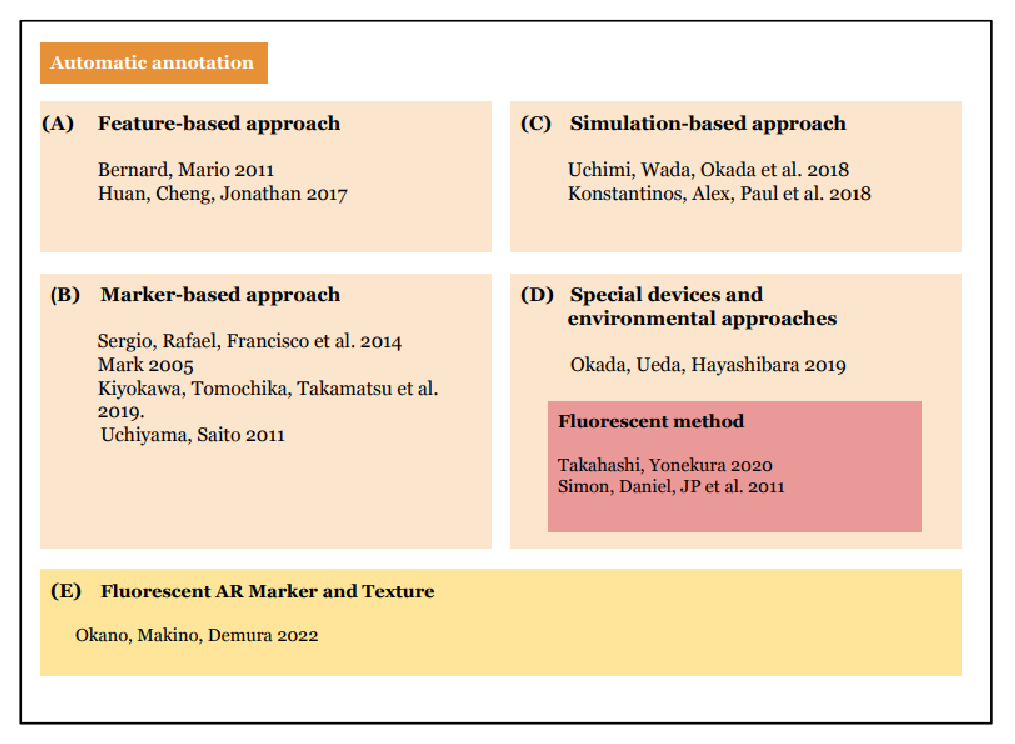
\includegraphics[width=160mm,clip]{figure/related_overview.eps}
\caption{Automatic annotation overview}
\label{Automatic annotation overview}
\end{center}
\end{figure*}

Fig. \ref{Automatic annotation overview}とFig. \ref{Automatic annotation overview using a Fluoresent AR marker}見てね!

\subsection{表の貼り方}
Table\ref{Hardware}を見てね!

\begin{table}[tb]
  \begin{center}
    \caption{{Equipment}\label{Hardware}}
    \scalebox{0.7}[0.9]{
      \begin{tabular}{|c|r|} \hline
        Microcomputer & Arduino Uno \\ \hline
        Motor & Dynamixel XM430-W350-R \\ \hline
        Communication converter & ROBOTIS, U2D2 SMPS2 \\ \hline
        Solid State Relays & Solid State Relays Kit Type 20A \\ \hline
        Visible light & Fluorescent LED light 40W \\ \hline
        UV light & TOSHIBA black light FL4BLB/N \\ \hline
        Camera & Realsense D435 \\ \hline
      \end{tabular}
    }
  \end{center}
\end{table}

\subsection{参考文献の引き方}
\cite{1}と\cite{2}を参考にする